% ZoonoMoE Conference Paper
% Springer LLNCS format — based on Springer_Lecture_Notes_in_Computer_Science template
%
\documentclass[runningheads]{llncs}
%
\usepackage[T1]{fontenc}
\usepackage[utf8]{inputenc}
\usepackage{graphicx}
\usepackage{amsmath}
\usepackage{booktabs}
\usepackage{array}
\usepackage{url}
\usepackage{tikz}
\usetikzlibrary{arrows.meta,positioning,fit,backgrounds,calc}
%
\begin{document}
%
\title{ZoonoMoE: A Voice-Driven Zoonotic Disease Surveillance System Using Mixture-of-Experts Routing and Domain-Partitioned Retrieval-Augmented Generation}
%
\titlerunning{A Specialist-Routing Cascade Architecture for Zoonotic Surveillance}
%
\author{Watin Promfiy\inst{1} \and Atibodee Kuiprasert\inst{1}}
%
\authorrunning{W. Promfiy and A. Kuiprasert}
%
\institute{King Mongkut's Institute of Technology Ladkrabang (KMITL), Bangkok, Thailand\\
\email{\{66070184,66070216\}@kmitl.ac.th}}
%
\maketitle
%
% ─────────────────────────────────────────────────────────────────────────────
\begin{abstract}
Zoonotic disease outbreaks represent a persistent threat to both animal and public health, particularly in agricultural communities where early detection is hampered by limited access to veterinary expertise. We present ZoonoMoE, an on-device, voice-driven surveillance pipeline that enables farmers and field workers to report suspected animal illness in natural speech and receive a structured veterinary risk assessment spoken back within seconds. The system integrates six AI components in sequence: (1) a bilingual Automatic Speech Recognition (ASR) module using OpenAI Whisper with automatic Thai-language routing to the Pathumma-whisper-th model; (2) a Large Language Model (LLM)-based Named Entity Recognition (NER) stage using Qwen3 to extract eight epidemiological fields; (3) a Mixture-of-Experts (MoE) Router combining sentence embeddings from all-MiniLM-L6-v2 with a two-layer MLP classifier to route reports into one of six disease domains (avian influenza, rabies, foot-and-mouth disease, Nipah/Hendra, leptospirosis, and general); (4) a domain-partitioned Retrieval-Augmented Generation (RAG) system with per-domain cosine vector stores backed by authoritative veterinary literature; (5) a domain-specific LLM expert agent built on Qwen3-4B that generates structured risk assessments via streaming inference; and (6) a Kokoro-82M text-to-speech module that synthesises audio sentence-by-sentence for low-latency spoken output. We benchmark the routing control plane against a spectrum of baselines under a single protocol; the corrected MLP classifier attains a macro F1 of \textbf{0.957} on a six-class cross-validation benchmark, and in doing so we surface and fix a deployment defect (early stopping on a small dataset) that had silently halved routing quality to 0.71. We further introduce a \emph{confidence-gated cascade} in which a sub-millisecond lexical classifier, calibrated by temperature scaling, answers most reports outright and escalates to the embedding model only when uncertain---matching the embedding router's accuracy while running the neural encoder on roughly 6\% of queries. All inference runs on-device using NVIDIA Triton Inference Server and vLLM, with no data leaving the local environment. ZoonoMoE demonstrates that a fully integrated, speech-in/speech-out AI pipeline can make expert-level zoonotic disease triage accessible to non-expert field users.

\keywords{Zoonotic disease surveillance \and Mixture-of-Experts routing \and Retrieval-Augmented Generation \and Automatic Speech Recognition \and Large Language Models \and On-device AI \and One Health}
\end{abstract}
%
% ─────────────────────────────────────────────────────────────────────────────
\section{Introduction}

State-of-the-art AI capabilities increasingly arise not from a single monolithic model but from \emph{compound systems}: pipelines that orchestrate multiple specialised models and retrieval components~\cite{compoundai}. Designing such systems raises architectural questions that are distinct from training any individual model---how components are composed, how control flows between them, how latency accumulates across a deep cascade, and how the whole is deployed under resource constraints. These questions are particularly acute for interactive, multimodal applications that must run \emph{on-device}, where neither unbounded compute nor cloud offload is available.

We study these questions through the lens of zoonotic disease surveillance. Zoonoses---diseases transmissible between animals and humans---account for over 60\% of emerging infectious diseases, with roughly 75\% of novel human pathogens originating in animal reservoirs~\cite{who_zoonoses}. Early recognition of abnormal mortality or morbidity in livestock is decisive for preventing spillover, yet trained veterinary expertise is scarce in the rural communities where outbreaks most often begin. Existing surveillance infrastructures, such as event-based aggregators~\cite{fao_empres,brownstein2008}, operate at the population level and do not provide individualised, point-of-observation triage. The interaction modalities that could close this gap---structured digital reporting forms---presuppose literacy, connectivity, and familiarity that exclude much of the at-risk population.

This setting imposes a demanding set of architectural constraints: the system must accept \emph{unstructured spoken} input in a low-resource language (Thai) alongside English; must produce an \emph{actionable, evidence-grounded} assessment rather than a free-form answer; must respond with \emph{low perceived latency} despite chaining several heavyweight models; and must run \emph{entirely on-device} for privacy and offline operability. No single model satisfies these constraints; a carefully composed architecture is required.

\paragraph{Contributions.}
We frame our contribution at the architectural level rather than as a single application:

\begin{enumerate}
    \item A \textbf{specialist-routing cascade architecture} for compound, on-device, speech-to-speech AI systems, expressed as a small set of design goals and principles (Sect.~\ref{sec:principles}) and a layered component decomposition (Sect.~\ref{sec:arch}).
    \item A \textbf{control-plane/data-plane separation} in which a lightweight, embedding-driven classifier acts as a control plane that conditions a shared generative backbone into one of several domain experts---achieving expert specialisation without replicating model weights.
    \item \textbf{Partition-aligned retrieval}, an architectural coupling in which the retrieval index topology is made congruent with the routing taxonomy, so that a single control decision selects both the expert persona and its evidence partition, eliminating cross-domain retrieval noise by construction.
    \item A \textbf{cross-cutting realisation strategy} (Sect.~\ref{sec:concerns}) addressing latency hiding via sentence-granular streaming, a hardware-adaptive serving model, and explicit graceful-degradation paths.
    \item A \textbf{confidence-gated cascade} for the control plane that makes routing cost adaptive: a calibrated lexical classifier resolves easy reports in under a millisecond and escalates to the embedding model only when uncertain, matching its accuracy at a fraction of the average cost (Sect.~\ref{sec:cascade}).
    \item An \textbf{instantiation and controlled evaluation} (ZoonoMoE) over six zoonotic domains that benchmarks the control plane against eight baselines, diagnoses and repairs a routing-quality regression, and quantifies the accuracy/cost and calibration trade-offs of the cascade.
\end{enumerate}

% ─────────────────────────────────────────────────────────────────────────────
\section{Background and Related Work}

\subsection{Compound and Modular AI Architectures}

The shift ``from models to compound AI systems''~\cite{compoundai} reframes capability as a property of an orchestrated pipeline. Retrieval-augmented generation (RAG)~\cite{lewis2020} is the canonical example, conditioning a generator on retrieved evidence to improve factuality. Our architecture extends this lineage with two structural commitments absent from a flat RAG pipeline: an explicit routing control plane upstream of retrieval, and a retrieval substrate whose partitioning is dictated by that control plane.

\subsection{Routing and Mixture-of-Experts}

Sparsely-gated Mixture-of-Experts (MoE) layers~\cite{shazeer2017} and MoE language models such as Mixtral~\cite{mixtral} route tokens through specialised sub-networks \emph{within} a model. We apply the same principle at the \emph{system} granularity: a classifier routes an entire request to a domain expert, instantiated through prompt and context conditioning rather than distinct weight sets. This is related to model- and prompt-routing work~\cite{lu2023}, but our router is grounded in sentence embeddings and is co-designed with the retrieval index it indexes into, rather than acting as a stand-alone selector. Our confidence-gated variant (Sect.~\ref{sec:cascade}) further connects to \emph{adaptive computation}: classifier cascades~\cite{viola2001} and early-exit networks~\cite{teerapittayanon2016} that spend compute in proportion to input difficulty, made reliable here through confidence calibration~\cite{guo2017}.

\subsection{Speech and Information-Extraction Components}

Whisper~\cite{radford2023} provides robust multilingual ASR via large-scale weak supervision; for Thai, the Pathumma-whisper-th model~\cite{pathumma} adapts it to local speech. LLM-based clinical information extraction~\cite{agrawal2022} demonstrates that structured fields can be extracted by prompting alone, avoiding task-specific training. Efficient LLM serving with continuous batching and PagedAttention~\cite{kwon2023} underpins the data plane's throughput. Our work treats each of these as an interchangeable component behind a stable interface, and contributes the \emph{composition} that binds them into a coherent, low-latency, on-device whole.

% ─────────────────────────────────────────────────────────────────────────────
\section{Design Goals and Architectural Principles}
\label{sec:principles}

We state the design goals the architecture must satisfy and the principles by which it satisfies them; the instantiation (Sect.~\ref{sec:arch}) follows directly.

\paragraph{Design goals.}
\textbf{G1 (Accessibility):} accept unstructured, bilingual spoken input and return spoken output, requiring no literacy or form-filling. \textbf{G2 (Groundedness):} condition assessments on authoritative domain evidence, emitted in a structured, decision-oriented form. \textbf{G3 (Responsiveness):} keep perceived latency low despite a deep cascade of heavyweight models. \textbf{G4 (On-device operability):} run entirely locally across heterogeneous hardware, with no cloud dependence.

\paragraph{Architectural principles.}
\textbf{P1 (Cascaded specialisation):} a monotone cascade in which each stage adds structure---\emph{audio} $\rightarrow$ \emph{text} $\rightarrow$ \emph{fields} $\rightarrow$ \emph{domain} $\rightarrow$ \emph{evidence} $\rightarrow$ \emph{assessment} $\rightarrow$ \emph{audio}---each a self-contained module with a typed interface, independently substitutable (G1, G4). \textbf{P2 (Control/data-plane separation):} a lightweight classifier (control plane) decides \emph{how} the data plane is configured---which expert persona and which evidence partition---so specialisation conditions a shared backbone rather than maintaining $N$ generators (G2, G4). \textbf{P3 (Partition-aligned retrieval):} the index is partitioned along the taxonomy the control plane classifies into, so the routing decision \emph{is} the retrieval selector and cross-domain contamination is precluded structurally, not filtered (G2). \textbf{P4 (Latency hiding):} adjacent stages overlap at sub-response granularity---synthesis of one sentence proceeds while the generator produces the next---decoupling first-output latency from response length (G3). \textbf{P5 (Hardware-adaptive realisation):} logical components bind to physical backends chosen at runtime, and every learned component has a training-free or reduced fallback for graceful degradation (G4).

% ─────────────────────────────────────────────────────────────────────────────
\section{System Architecture}
\label{sec:arch}

The architecture is a six-stage cascade (Fig.~\ref{fig:pipeline}) governed by the principles of Sect.~\ref{sec:principles}. We describe each stage as a module defined by its interface contract and architectural role; implementation details are deferred to Sect.~\ref{sec:concerns}.

\begin{figure}[t]
\centering
\resizebox{\textwidth}{!}{%
\begin{tikzpicture}[
  font=\small,
  node distance=9mm,
  box/.style={draw, rounded corners, minimum height=11mm, minimum width=15mm,
              align=center, fill=white},
  io/.style={draw, ellipse, minimum height=9mm, minimum width=13mm,
             align=center, fill=black!4},
  ctrl/.style={draw, thick, rounded corners, minimum height=12mm, minimum width=30mm,
               align=center, fill=black!8},
  flow/.style={-{Stealth[length=2.4mm]}, thick},
  cond/.style={-{Stealth[length=2mm]}, dashed, draw=black!55},
]
% ── data plane (bottom chain) ────────────────────────────────────────────────
\node[io]  (voice)                  {voice};
\node[box, right=of voice] (asr)    {ASR\\{\scriptsize Stage 1}};
\node[box, right=of asr]   (ner)    {NER\\{\scriptsize Stage 2}};
\node[box, right=of ner]   (rag)    {RAG$_d$\\{\scriptsize Stage 4}};
\node[box, right=of rag]   (exp)    {Expert$_d$\\{\scriptsize Stage 5}};
\node[box, right=of exp]   (tts)    {TTS$_d$\\{\scriptsize Stage 6}};
\node[io, right=of tts]    (speech) {speech};

\draw[flow] (voice) -- (asr);
\draw[flow] (asr)   -- (ner);
\draw[flow] (ner)   -- (rag);
\draw[flow] (rag)   -- (exp);
\draw[flow] (exp)   -- (tts);
\draw[flow] (tts)   -- (speech);

% ── control plane (router above) ─────────────────────────────────────────────
\coordinate (cmid) at ($(ner)!0.5!(rag)$);
\node[ctrl, above=16mm of cmid] (router)
      {Router \textbf{(Stage 3)}\\{\scriptsize classifies report $\;\Rightarrow\; d$}};

% control signal in, conditioning out
\draw[flow] (ner.north) |- (router.south);
\draw[cond] (router.south) to[out=-90,in=90] (rag.north);
\draw[cond] (router.south) to[out=-90,in=90] (exp.north);
\draw[cond] (router.south) to[out=-90,in=90] (tts.north)
      node[pos=0.55, right, font=\scriptsize, black!60] {domain $d$};

% ── plane backgrounds ────────────────────────────────────────────────────────
\begin{scope}[on background layer]
  \node[fit=(voice)(speech), draw=black!25, rounded corners,
        inner sep=4mm, fill=black!2, label={[font=\scriptsize\itshape, black!60]
        below:data plane --- shared backbone, specialised by $d$}] {};
  \node[fit=(router), draw=black!25, rounded corners, inner sep=3mm,
        fill=black!4, label={[font=\scriptsize\itshape, black!60]
        above:control plane}] {};
\end{scope}
\end{tikzpicture}%
}
\caption{The specialist-routing cascade. The data plane (bottom) carries the signal
\texttt{voice}$\rightarrow$ASR$\rightarrow$NER$\rightarrow$RAG$\rightarrow$Expert$\rightarrow$TTS$\rightarrow$\texttt{speech}.
The control plane (Stage~3) classifies each report into a domain $d$ from the transcript
and extracted fields; this single decision conditions (dashed) the evidence partition
(Stage~4), the expert persona (Stage~5), and the synthesis voice (Stage~6). The data
plane is a shared backbone specialised by $d$ rather than $|\mathcal{D}|$ separate
models. All stages run on-device.}
\label{fig:pipeline}
\end{figure}

\subsection{Stage 1 --- Bilingual Speech Recognition (Signal $\rightarrow$ Text)}

\emph{Interface:} audio buffer $\mapsto$ transcript $\in \Sigma^{*}$.
The module realises a two-pass strategy that internalises language identification: a base recogniser~\cite{radford2023} first estimates a language posterior from the mel spectrogram; Thai input is dispatched to a Thai-adapted recogniser~\cite{pathumma}, otherwise the base model transcribes directly. This satisfies G1 (bilingual access) behind a single language-agnostic interface. A robustness contract guards the cascade against degenerate input: transcripts exhibiting pathological repetition (a token run exceeding six, or a top-3 token mass above 0.8) are rejected at the source rather than propagated downstream, embodying a fail-fast boundary that prevents error amplification through the deep cascade.

\subsection{Stage 2 --- Epidemiological Extraction (Text $\rightarrow$ Structured Fields)}

\emph{Interface:} transcript $\mapsto$ record $r$ with eight typed fields
(\texttt{species}, \texttt{symptoms}, \texttt{mortality\_count}, \texttt{affected\_count},
\texttt{location}, \texttt{timeframe}, \texttt{reporter\_role}, \texttt{raw\_summary}).
Extraction is performed by constrained, JSON-mode prompting of a general language model, with chain-of-thought spans stripped and a schema-conformant default returned on parse failure. Architecturally, the choice of prompting over a fine-tuned extractor is deliberate (Sect.~\ref{sec:tradeoffs}): it keeps the module training-free and tolerant of paraphrase and code-switching, consistent with P5. The structured record $r$ serves two consumers: it enriches the control plane (Sect.~\ref{sec:control}) and conditions the data-plane expert (Sect.~\ref{sec:expert}).

\subsection{Stage 3 --- The Routing Control Plane (Fields + Text $\rightarrow$ Domain)}
\label{sec:control}

The control plane maps a report to a domain $d \in \mathcal{D}$, where $\mathcal{D}$ comprises the dominant regional zoonoses---avian influenza, rabies, foot-and-mouth disease, Nipah/Hendra, leptospirosis---and a \texttt{general} category. It is the architecture's locus of decision and the realisation of P2.

\paragraph{Control-signal enrichment.}
Rather than classifying raw text, the control plane fuses the conversational transcript with the structured clinical vocabulary extracted in Stage~2:
\begin{equation}
q_{\text{enriched}} = \text{transcript} \,\|\, \texttt{``Species: ''}{+}s \,\|\, \texttt{``Symptoms: ''}{+}y,
\end{equation}
with $s$ the species list and $y$ the top symptoms. This couples the control plane to upstream structure at zero additional parameter cost.

\paragraph{Embedding and classification.}
The enriched query is encoded by a sentence encoder~\cite{reimers2019} into an $L_2$-normalised $\mathbf{e}\in\mathbb{R}^{384}$. A two-layer MLP forms the primary classifier,
\begin{equation}
P(d\mid\mathbf{e}) = \mathrm{softmax}\!\big(W_2\,\mathrm{ReLU}(W_1\mathbf{e}+b_1)+b_2\big),\quad W_1\in\mathbb{R}^{128\times384},\,W_2\in\mathbb{R}^{6\times64}.
\end{equation}
Per P5, the control plane degrades gracefully: when no trained classifier is present, it falls back to a training-free nearest-centroid rule over per-domain seed centroids $\bar{\mathbf{c}}_d$ with temperature-scaled cosine scores,
\begin{equation}
P(d\mid\mathbf{e}) = \frac{\exp(\tau\,\mathbf{e}^{\top}\bar{\mathbf{c}}_d)}{\sum_{d'}\exp(\tau\,\mathbf{e}^{\top}\bar{\mathbf{c}}_{d'})},\qquad \tau=10,
\end{equation}
so the system is deployable in a new environment before any training data exists.

\paragraph{Scope gating.}
A guard short-circuits the expert pipeline for inputs that fall outside the surveillance scope: low classifier confidence ($<0.35$) combined with an absence of clinical entities (no extracted species or symptoms), or a lexical match against conversational openers, reroutes the request to a lightweight advisory mode. This protects the data plane from running an assessment over irrelevant input.

\paragraph{Adaptive routing cost.}
The MLP and centroid paths both pay for the sentence encoder. Since the encoder dominates routing cost while a far cheaper lexical model already suffices on unambiguous reports, the control plane can be operated as a \emph{confidence-gated cascade} that invokes the encoder only when a calibrated cheap stage is uncertain. We develop and evaluate this in Sect.~\ref{sec:cascade}.

\subsection{Stage 4 --- Partition-Aligned Retrieval (Domain $\rightarrow$ Evidence)}

\emph{Interface:} (query, domain $d$) $\mapsto$ top-$k$ evidence chunks.
Realising P3, the knowledge substrate is decomposed into one independent vector store per domain. Retrieval is confined to the partition the control plane selected:
\begin{equation}
\mathrm{top\text{-}}k \;=\; \operatorname*{arg\,top\text{-}}k_{\,i\in d}\;\frac{\mathbf{q}^{\top}\mathbf{v}_i}{\lVert\mathbf{q}\rVert\,\lVert\mathbf{v}_i\rVert}.
\end{equation}
Because the index topology is congruent with the routing taxonomy, cross-domain retrieval is impossible by construction rather than suppressed by score thresholding: a query routed to \texttt{avian\_flu} can never surface leptospirosis evidence, even under lexical overlap (e.g.\ shared mentions of flooding or livestock). Each partition is seeded from authoritative veterinary and public-health sources; the module exposes the same interface whether backed by a persisted index or an embedded seed corpus, preserving operability under G4.

\subsection{Stage 5 --- The Conditioned Expert (Evidence + Fields $\rightarrow$ Assessment)}
\label{sec:expert}

\emph{Interface:} (domain $d$, record $r$, evidence) $\mapsto$ structured assessment stream.
The data plane attains expert behaviour by \emph{conditioning a single shared generator}, not by hosting $|\mathcal{D}|$ models (P2). The control decision selects (a) a domain persona, (b) the retrieved evidence, and (c) the structured record, which are composed into a system prompt that constrains the output to a fixed decision schema---clinical assessment, an ordinal risk level (\textsc{low}/\textsc{medium}/\textsc{high}/\textsc{critical}), immediate actions, handling, reporting obligation, and human-safety guidance---satisfying G2. The risk level and a reporting flag are parsed from the stream as structured side-channels for the user interface. This conditioning-based specialisation is what makes the architecture tractable on a single device: domain breadth scales with prompt and index entries, not with resident model weights.

\subsection{Stage 6 --- Streaming Synthesis (Assessment $\rightarrow$ Speech)}

\emph{Interface:} assessment text stream $\mapsto$ audio chunk stream.
The synthesis module consumes the generator's token stream through a sentence-boundary segmenter and emits audio per completed sentence, realising the producer side of P4. Each chunk is streamed to a sequential playback buffer, and the voice is selected by domain $d$, closing the loop on the control plane's decision. A pre-synthesis normalisation step removes formatting artefacts and expands domain abbreviations to improve prosody.

% ─────────────────────────────────────────────────────────────────────────────
\section{Cross-Cutting Architectural Concerns}
\label{sec:concerns}

The stage decomposition above defines \emph{what} the components are; this section addresses the system-level properties that emerge from \emph{how} they are composed and realised.

\subsection{Control Plane vs.\ Data Plane}

Separating a cheap, fast classifier (the control plane) from the expensive generative and retrieval components (the data plane) yields three architectural benefits. First, the routing decision is computed once and reused to configure three downstream stages (evidence, persona, voice), amortising a single inference across the cascade. Second, the planes evolve independently: domains can be added by extending the taxonomy, seeding a partition, and supplying routing exemplars---without retraining or replicating the generator. Third, the scope gate (Sect.~\ref{sec:control}) lets the control plane veto data-plane execution entirely, bounding cost on out-of-scope input.

\subsection{Serving Topology and Concurrency}

The realisation maps logical stages onto a heterogeneous serving substrate. Stateless, CPU-bound components (ASR, the sentence encoder, synthesis) are hosted as independently scaled instance groups on an inference server, so that, e.g., multiple syntheses proceed in parallel. The generator is served by an engine providing continuous batching and PagedAttention~\cite{kwon2023}, which interleaves concurrent requests internally; it is therefore \emph{not} placed behind the generic instance-group mechanism, since doing so would impose decoupled-streaming complexity without throughput benefit. This asymmetry---instance-group replication for stateless modules, internal batching for the generator---is a deliberate consequence of each component's concurrency model.

\subsection{Latency Hiding}

Total cascade latency is the sum of stage latencies, but \emph{perceived} latency is governed by time-to-first-output. P4 exploits the fact that the two longest stages---generation and synthesis---can be pipelined at sentence granularity. First audio is emitted after the first complete sentence rather than the full assessment, decoupling the user's wait from the response length and keeping the interaction within conversational tolerance (G3).

\subsection{Hardware-Adaptive Realisation}

Per P5, logical components bind to physical backends chosen at runtime by hardware capability (Table~\ref{tab:llm_backend}). The same architecture runs on Apple Silicon, discrete GPUs of differing compute capability, and CPU-only hosts, with precision and model size adjusted accordingly. Combined with the control plane's centroid fallback and the retrieval module's seed-corpus fallback, this yields a system that is portable across deployment targets and degrades along well-defined axes rather than failing.

\begin{table}[t]
\caption{Hardware-adaptive binding of the generative backend (illustrative).}\label{tab:llm_backend}
\centering
\begin{tabular}{llll}
\toprule
Platform & Model class & Serving backend & Precision \\
\midrule
Apple Silicon & 4B (quantised) & on-device runtime & 4-bit \\
GPU (cc$\geq$8.0) & 4B & batched engine & FP16 \\
GPU (cc$=$7.5) & 4B (AWQ) & batched engine & INT8 \\
CPU only & 1.5B & batched engine & FP32 \\
\bottomrule
\end{tabular}
\end{table}

% ─────────────────────────────────────────────────────────────────────────────
\section{Evaluation}

We evaluate the architecture along three axes: the quality of the control plane, which is the decision point on which all downstream specialisation depends; the accuracy/cost and calibration trade-off of routing it as a confidence-gated cascade; and the responsiveness of the streamed data plane.

\subsection{Control-Plane Routing Quality}

The router is assessed by 5-fold stratified cross-validation (seed 42) over a labelled benchmark of 160 short reports balanced across the six domains (counts: \texttt{avian\_flu} 27, \texttt{rabies} 27, \texttt{fmd} 25, \texttt{nipah\_hendra} 30, \texttt{leptospirosis} 26, \texttt{general} 25). The benchmark is semi-synthetic: report templates were adapted from publicly reported outbreak descriptions and lexically diversified to broaden surface form. Because every downstream stage is conditioned on the routing decision, routing quality upper-bounds end-to-end specialisation, making it the architecture's principal quantitative target.

\paragraph{A deployment defect and its repair.}
The MLP classifier originally shipped with scikit-learn early stopping and a 15\% internal validation split. On 160 examples this configuration halts optimisation before the network fits the task, collapsing macro F1 to $0.707\pm0.265$---worse than a keyword baseline, with extreme fold variance. Disabling early stopping with mild $L_2$ regularisation recovers $0.95$--$0.96$ independently of hidden width. This is a reproducible cautionary instance of a default that is benign at scale but harmful on small data; the corrected configuration is the deployed model. We report it because the control plane is the architecture's leverage point, and the regression would otherwise silently bound every downstream stage.

\paragraph{Baselines and the cost of routing.}
We benchmark the control plane against a spectrum of alternatives under one protocol that reports both accuracy and deployment cost (Table~\ref{tab:router_baselines}): a majority floor, hand-written keyword rules, TF--IDF with logistic regression, and four heads on the shared sentence embeddings (nearest-centroid, $k$-NN, logistic regression, and the MLP). Two observations follow. First, every embedding head with a sound configuration clusters near $0.94$--$0.96$ macro F1, statistically indistinguishable, confirming that a kilobyte-scale linear head suffices and an LLM call per query is unnecessary for routing. Second, the dominant cost is the shared encoder ($\sim$14\,ms), not the classifier ($<0.3$\,ms); a purely lexical TF--IDF model already reaches $0.95$ at sub-millisecond cost, which we exploit in Sect.~\ref{sec:cascade}.

\begin{table}[t]
\caption{Six-way routing: 5-fold stratified CV (seed 42, $n{=}160$). Latency is the median per query on one CPU thread (encoder $+$ classifier for embedding methods); model size is the serialised classifier (the shared encoder, $\sim$90\,MB, is amortised across embedding methods).}\label{tab:router_baselines}
\centering
\begin{tabular}{lcccc}
\toprule
Method & Macro F1 & Accuracy & Latency (ms) & Size \\
\midrule
Majority (floor)            & $0.053$            & $0.188$ & ---    & ---     \\
Keyword / regex             & $0.817$            & $0.825$ & $0.01$ & ---     \\
TF--IDF $+$ LogReg          & $0.948\pm0.039$    & $0.950$ & $0.8$  & $147$\,KB \\
Nearest centroid (cosine)   & $0.936\pm0.044$    & $0.938$ & $13.8$ & $10$\,KB  \\
$k$-NN ($k{=}5$)            & $0.943\pm0.033$    & $0.944$ & $15.0$ & $242$\,KB \\
LogReg (embedding)          & $0.943\pm0.048$    & $0.944$ & $13.8$ & $19$\,KB  \\
MLP $(128,64)$ early-stop   & $0.707\pm0.265$    & $0.744$ & $13.9$ & $687$\,KB \\
\textbf{MLP $(64)$ [ours]}  & $\mathbf{0.956\pm0.033}$ & $\mathbf{0.956}$ & $14.0$ & $405$\,KB \\
\bottomrule
\end{tabular}
\end{table}

\begin{figure}[t]
\centering
\begin{minipage}[t]{0.49\textwidth}
\centering
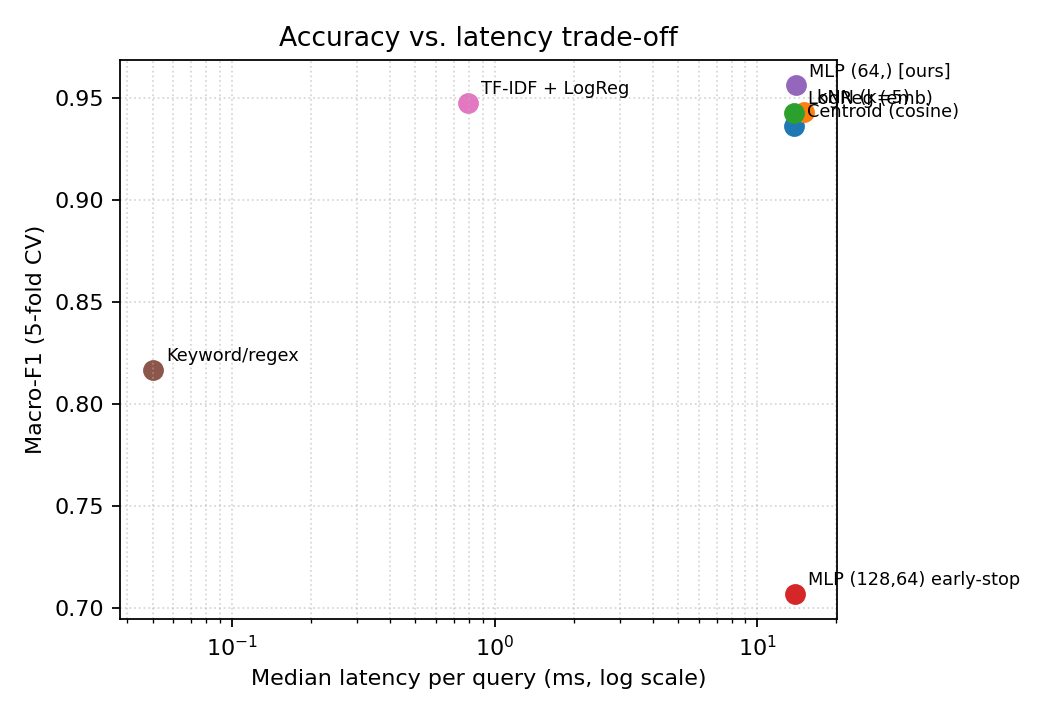
\includegraphics[width=\textwidth]{pareto.png}
\caption{Accuracy vs.\ latency for all routing methods (log-scale latency). Embedding heads share the $\sim$14\,ms encoder cost; the lexical baselines sit far to the left.}
\label{fig:pareto-baselines}
\end{minipage}\hfill
\begin{minipage}[t]{0.49\textwidth}
\centering
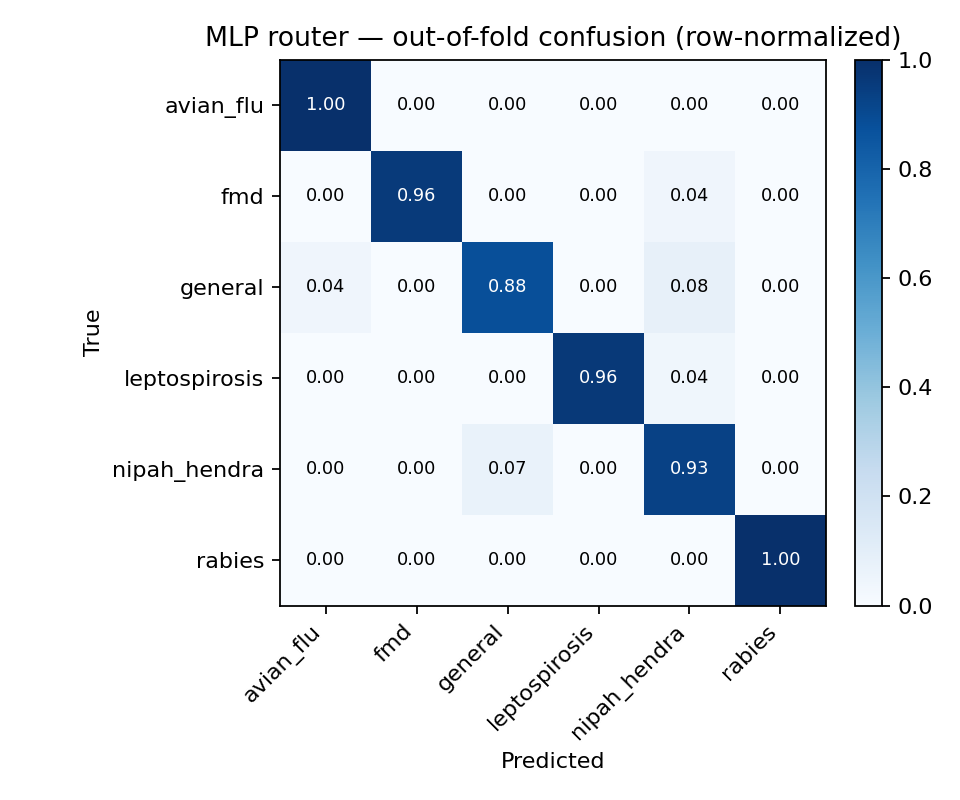
\includegraphics[width=\textwidth]{confusion_matrix.png}
\caption{Out-of-fold, row-normalised confusion matrix for the corrected router. Residual errors concentrate between epidemiologically adjacent domains and the catch-all \texttt{general} class.}
\label{fig:confusion}
\end{minipage}
\end{figure}

The accuracy/cost picture is shown in Fig.~\ref{fig:pareto-baselines}, and the corrected router's error structure in Fig.~\ref{fig:confusion}: misroutes are confined to neighbouring domains (e.g.\ \texttt{general} vs.\ specific diseases) rather than distributed arbitrarily, which is the benign failure mode for a control plane feeding partition-aligned retrieval.

\subsection{Confidence-Gated Cascade Routing}
\label{sec:cascade}

The baseline analysis exposes an asymmetry: the embedding encoder dominates routing cost ($\sim$14\,ms) yet a lexical model already reaches $0.95$ at $<$1\,ms. This motivates making the control plane's cost \emph{adaptive}. We add a two-stage cascade: Stage~1 is the TF--IDF$+$LogReg classifier; Stage~2 is the corrected embedding$+$MLP router. Stage~1 answers when its confidence exceeds a threshold $\tau$; otherwise the request escalates to Stage~2. Because a gate is only as good as the confidence it trusts, we calibrate Stage~1 by \emph{temperature scaling}~\cite{guo2017}---a single scalar $T$ fit by minimising negative log-likelihood on a held-out split, replacing $\mathrm{softmax}(z)$ with $\mathrm{softmax}(z/T)$. To prevent leakage, within each outer CV fold both stages are trained on the training portion, $T$ is fit on an inner calibration split, and metrics are computed on the untouched test fold.

Temperature scaling reduces Stage~1 expected calibration error (ECE) from $0.385$ to $0.040$ ($T\!\approx\!0.26$; Fig.~\ref{fig:reliability}), making the gate trustworthy. The calibrated cascade then dominates both single-stage routers (Table~\ref{tab:cascade}, Fig.~\ref{fig:cascade}): at $\tau{=}0.54$ it matches---in fact marginally exceeds, via a mild ensemble effect---the Stage~2 macro F1 ($0.969$ vs.\ $0.957$) while escalating only $\sim$6\% of queries, giving an average routing latency of $1.29$\,ms, roughly a $90\%$ reduction versus always invoking the encoder. The frontier is flat over a wide $\tau$ range, so the operating point is not brittle. This is P4's latency-hiding philosophy applied to the control plane itself: spend compute in proportion to input difficulty.

\begin{table}[t]
\caption{Confidence-gated cascade vs.\ single-stage routers (5-fold CV). Average latency assumes the encoder runs only on escalated queries.}\label{tab:cascade}
\centering
\begin{tabular}{lcccc}
\toprule
Router & Macro F1 & Accuracy & Avg.\ latency (ms) & Escalation \\
\midrule
Stage 1 only (TF--IDF$+$LogReg)   & $0.923$ & $0.925$ & $0.58$  & $0\%$   \\
Stage 2 only (embedding$+$MLP)    & $0.957$ & $0.956$ & $13.19$ & $100\%$ \\
\textbf{Cascade ($\tau{=}0.54$)}  & $\mathbf{0.969}$ & $\mathbf{0.969}$ & $\mathbf{1.29}$ & $6\%$ \\
Cascade ($\tau{=}0.78$, max-F1)   & $0.970$ & $0.969$ & $1.92$  & $11\%$  \\
\bottomrule
\end{tabular}
\end{table}

\begin{figure}[t]
\centering
\begin{minipage}[t]{0.49\textwidth}
\centering
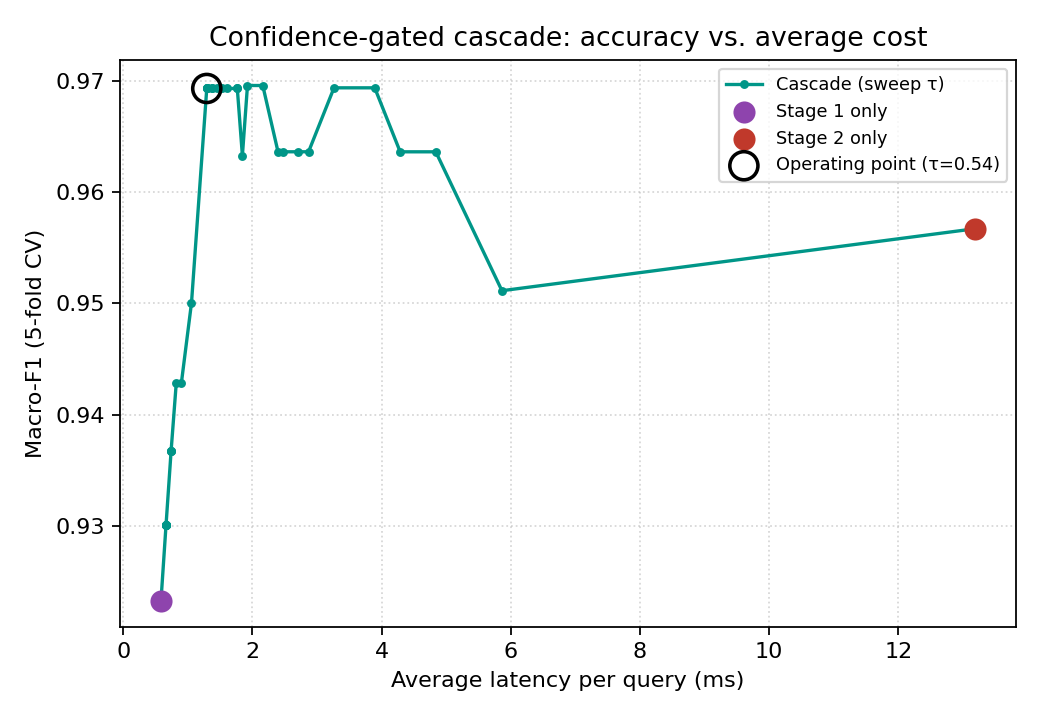
\includegraphics[width=\textwidth]{cascade_pareto.png}
\caption{Cascade accuracy vs.\ average latency as $\tau$ sweeps; the operating point matches Stage-2 accuracy at a fraction of its cost.}
\label{fig:cascade}
\end{minipage}\hfill
\begin{minipage}[t]{0.49\textwidth}
\centering
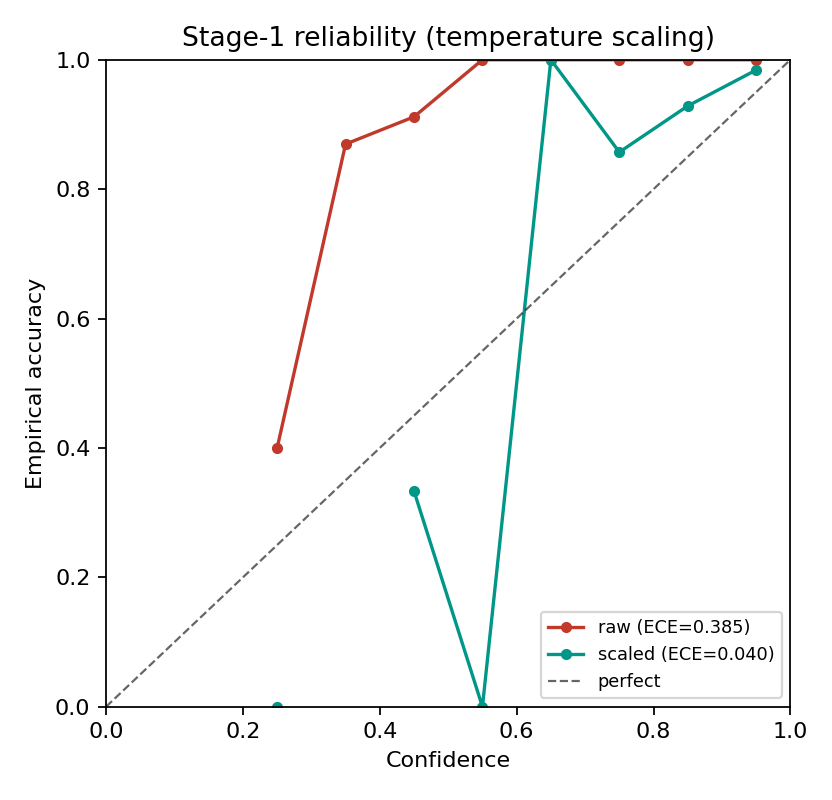
\includegraphics[width=\textwidth]{reliability.png}
\caption{Stage-1 reliability before/after temperature scaling (ECE $0.385\!\to\!0.040$).}
\label{fig:reliability}
\end{minipage}
\end{figure}

\subsection{Ablations: Classifier Head and Embedding Backbone}

We isolate the two design choices internal to the control plane: the classifier head atop the frozen embedding, and the embedding backbone itself.

\paragraph{Classifier head (Table~\ref{tab:ablA}).}
Holding the encoder fixed at \texttt{all-MiniLM-L6-v2}, we sweep heads. The result is unambiguous: \emph{what matters is not capacity but the early-stopping defect}. The deployed-as-shipped MLP collapses to $0.707$, while every other configuration---an MLP without early stopping at three widths, logistic regression, a linear SVM, $k$-NN, and a nearest-centroid rule---lands within a narrow $0.936$--$0.956$ band. Capacity is therefore essentially free to choose; we select the smallest competitive MLP, $(64)$, at $0.956$. The training-free nearest-centroid rule reaching $0.936$ is what makes the P5 zero-shot fallback (Sect.~\ref{sec:control}) viable: a fresh deployment is usefully accurate before any labelled data exists.

\begin{table}[t]
\caption{Ablation A: classifier head on frozen \texttt{all-MiniLM-L6-v2} (5-fold CV). Removing early stopping is decisive; head capacity is not.}\label{tab:ablA}
\centering
\begin{tabular}{lcc}
\toprule
Head & Macro F1 & Accuracy \\
\midrule
MLP $(128,64)$ early-stop [as shipped] & $0.707\pm0.265$ & $0.744$ \\
MLP $(128,64)$ no early-stop           & $0.950\pm0.037$ & $0.950$ \\
MLP $(256)$ no early-stop              & $0.950\pm0.038$ & $0.950$ \\
\textbf{MLP $(64)$ no early-stop [ours]} & $\mathbf{0.956\pm0.033}$ & $\mathbf{0.956}$ \\
Logistic regression                    & $0.943\pm0.048$ & $0.944$ \\
Linear SVM                             & $0.942\pm0.048$ & $0.944$ \\
$k$-NN ($k{=}5$, cosine)               & $0.943\pm0.033$ & $0.944$ \\
Nearest centroid (cosine)              & $0.936\pm0.044$ & $0.938$ \\
\bottomrule
\end{tabular}
\end{table}

\paragraph{Embedding backbone (Table~\ref{tab:ablB}).}
Fixing the head to logistic regression and varying the encoder, the three MiniLM variants---including a multilingual one---are within noise at $\sim$0.94, whereas \texttt{bge-small-en-v1.5}, at an identical 384 dimensions and comparable cost, lifts macro F1 to $0.969$. The control plane thus has a clear, cost-free upgrade path: a stronger same-size encoder improves routing without touching the rest of the architecture. We retain MiniLM in the deployed system for its maturity and multilingual sibling, noting BGE as a drop-in improvement.

\begin{table}[t]
\caption{Ablation B: embedding backbone, head fixed to logistic regression (5-fold CV). All encoders are 384-dimensional.}\label{tab:ablB}
\centering
\begin{tabular}{lcc}
\toprule
Backbone (384-d) & Macro F1 & Accuracy \\
\midrule
\texttt{all-MiniLM-L6-v2} [deployed]              & $0.943\pm0.048$ & $0.944$ \\
\texttt{all-MiniLM-L12-v2}                        & $0.942\pm0.048$ & $0.944$ \\
\texttt{paraphrase-multilingual-MiniLM-L12-v2}    & $0.942\pm0.055$ & $0.944$ \\
\texttt{bge-small-en-v1.5}                        & $\mathbf{0.969\pm0.040}$ & $\mathbf{0.969}$ \\
\bottomrule
\end{tabular}
\end{table}

\paragraph{Per-domain behaviour.}
Per-domain F1 is uniformly high (0.90--1.00); the two softest classes are \texttt{general} and \texttt{nipah\_hendra}, consistent with the confusion structure of Fig.~\ref{fig:confusion}: \texttt{general} is a deliberately broad catch-all, and \texttt{nipah\_hendra} shares pig/bat and febrile-worker vocabulary with neighbouring domains. Crucially, no domain is pathologically weak, so the single routing decision is a sound foundation for the downstream partition-aligned retrieval.

\subsection{Partition-Aligned Retrieval}

We measure precision@3 over a held-out set of domain-labelled queries, scoring a query as satisfied when at least two of three retrieved chunks originate from the correct partition. Under partition-aligned retrieval this is satisfied across the test queries by construction, confirming that P3 removes cross-domain noise as a category of error rather than reducing its frequency.

\subsection{Data-Plane Responsiveness}

The sentence-granular streaming of P4 yields a first spoken response within a few seconds of generation onset; on an NVIDIA A100 the full speech-to-speech cycle for a typical report completes in approximately 2--5\,s, dominated by expert-LLM generation and scaling with response length. The middle of the pipeline is comparatively negligible: NER, routing, and retrieval together account for well under two seconds, and the cascade keeps the routing stage itself in the millisecond range (Sect.~\ref{sec:cascade}). A detailed, instrumented per-stage breakdown (NER, router, RAG, time-to-first-token, expert LLM, TTS) is collected by a benchmark harness we release; full end-to-end timing tables are left to an extended version, as they depend on the specific GPU and decoding length.

\subsection{Qualitative Behaviour}

Across representative reports spanning all six domains---e.g.\ ``chickens dead, purple combs, twisted necks'' ($\rightarrow$\,\texttt{avian\_flu}, \textsc{critical}), ``cattle blisters on tongue and hooves, salivating'' ($\rightarrow$\,\texttt{fmd}, \textsc{high}), ``stray dog foaming, bit two children'' ($\rightarrow$\,\texttt{rabies}, \textsc{critical})---the control plane selects the correct partition, the data plane retrieves congruent evidence, and the emitted ordinal risk level is consistent with published veterinary guidance, including correct gating of an out-of-scope conversational query (``how do I protect myself near livestock?'') to the advisory mode.

% ─────────────────────────────────────────────────────────────────────────────
\section{Discussion: Architectural Trade-offs}
\label{sec:tradeoffs}

\paragraph{Partitioned vs.\ unified retrieval.}
Partition-aligned retrieval trades a small loss of cross-domain recall for the structural elimination of cross-domain noise. In a surveillance setting, where a confidently misleading retrieval is more harmful than a missed tangential one, this favours partitioning---at the cost of making retrieval quality contingent on routing correctness, concentrating risk at the control plane.

\paragraph{Conditioned experts vs.\ specialised models.}
Conditioning a shared backbone (P2) keeps the resident footprint constant as domains grow, making on-device breadth feasible (G4); the cost is that all experts inherit the backbone's competence and cannot diverge beyond what prompt and evidence conditioning express. For deep specialisation this ceiling may bind; for triage-level guidance it is acceptable.

\paragraph{Prompted vs.\ trained extraction.}
LLM-based extraction (Stage~2) avoids annotation and absorbs paraphrase and code-switching, at the price of latency and unpredictability on rare entities---severe enough that it is bypassed on the weakest hardware tier, a concrete instance of P5's degradation axis.

\paragraph{Limitations and future work.}
While the corrected router reaches $0.957$ macro F1, this is measured on a small ($n{=}160$), semi-synthetic, single-region, English-only benchmark; absolute figures should be read as relative comparisons under a fixed protocol, and with so few examples the high-confidence calibration bins are sparse, so $\tau$ should be re-tuned on a larger calibration set before deployment. An active-learning loop---routing escalated (low-confidence) requests to human adjudication and incrementally retraining---would both raise the ceiling and tune $\tau$ from the deployment itself. A full instrumented end-to-end timing study across hardware tiers, a formal partitioned-vs-unified retrieval ablation, and a genuinely multilingual (Thai) evaluation are natural next steps.

% ─────────────────────────────────────────────────────────────────────────────
\section{Conclusion}

We presented a specialist-routing cascade architecture for compound, on-device, speech-to-speech AI systems, distilled into four design principles---cascaded specialisation, control/data-plane separation, partition-aligned retrieval, and streaming latency hiding---realised in a hardware-adaptive manner with explicit graceful degradation. Instantiated as ZoonoMoE over six zoonotic disease domains, the architecture delivers grounded, spoken triage to non-expert field users entirely on-device, with a corrected control plane attaining $0.957$ macro F1---and, via a calibrated confidence-gated cascade, matching that accuracy while invoking the embedding encoder on only $\sim$6\% of queries---and a streamed data plane responding within a few seconds of generation onset. The central architectural insight is that aligning a lightweight control plane with a partitioned retrieval substrate---so that one routing decision configures evidence, persona, and voice in concert---yields expert specialisation without per-domain model replication, an effective and portable pattern for compound AI systems under tight resource constraints.

% ─────────────────────────────────────────────────────────────────────────────
\begin{credits}
\subsubsection{\ackname}
The authors thank the Department of Livestock Development (DLD) of Thailand for domain guidance.

\subsubsection{\discintname}
The authors have no competing interests to declare that are relevant to the content of this article.
\end{credits}

% ─────────────────────────────────────────────────────────────────────────────
% \bibliographystyle{splncs04}
% \bibliography{references}

\begin{thebibliography}{20}

\bibitem{compoundai}
Zaharia, M., Khattab, O., Chen, L., Davis, J.Q., Miller, H., Potts, C.,
Zou, J., Carbin, M., Frankle, J., Rao, N., Ghodsi, A.:
The Shift from Models to Compound AI Systems.
Berkeley Artificial Intelligence Research (BAIR) Blog (2024).
\url{https://bair.berkeley.edu/blog/2024/02/18/compound-ai-systems/},
last accessed 2025/12/01

\bibitem{who_zoonoses}
World Health Organization: Zoonoses. WHO Fact Sheet (2023).
\url{https://www.who.int/news-room/fact-sheets/detail/zoonoses},
last accessed 2025/12/01

\bibitem{fao_empres}
Food and Agriculture Organization: EMPRES-i Global Animal Disease
Information System. FAO (2024).
\url{https://empres-i.apps.fao.org/}, last accessed 2025/12/01

\bibitem{brownstein2008}
Brownstein, J.S., Freifeld, C.C., Reis, B.Y., Mandl, K.D.:
Surveillance Sans Fronti\`{e}res: Internet-Based Emerging Infectious
Disease Intelligence and the HealthMap Project.
PLOS Medicine \textbf{5}(7), e151 (2008). \doi{10.1371/journal.pmed.0050151}

\bibitem{lewis2020}
Lewis, P., et al.: Retrieval-Augmented Generation for
Knowledge-Intensive NLP Tasks.
In: Advances in Neural Information Processing Systems (NeurIPS 2020),
vol.~33, pp.~9459--9474 (2020)

\bibitem{shazeer2017}
Shazeer, N., et al.: Outrageously Large Neural Networks: The
Sparsely-Gated Mixture-of-Experts Layer.
In: International Conference on Learning Representations (ICLR 2017) (2017)

\bibitem{mixtral}
Jiang, A.Q., et al.: Mixtral of Experts. arXiv:2401.04088 (2024)

\bibitem{lu2023}
Lu, K., et al.: Routing to the Expert: Efficient Reward-Guided
Ensemble of Large Language Models. arXiv:2311.08692 (2023)

\bibitem{radford2023}
Radford, A., Kim, J.W., Xu, T., Brockman, G., McLeavey, C., Sutskever, I.:
Robust Speech Recognition via Large-Scale Weak Supervision.
In: Proceedings of the 40th International Conference on Machine Learning
(ICML 2023), PMLR \textbf{202}, pp.~28492--28518 (2023)

\bibitem{pathumma}
NECTEC: Pathumma-whisper-th --- Thai Automatic Speech Recognition Model.
National Electronics and Computer Technology Center, Thailand (2024).
\url{https://huggingface.co/nectec/Pathumma-whisper-th-medium},
last accessed 2025/12/01

\bibitem{agrawal2022}
Agrawal, M., et al.: Large Language Models are Few-Shot Clinical
Information Extractors.
In: Proceedings of the 2022 Conference on Empirical Methods in Natural
Language Processing (EMNLP 2022), pp.~1998--2022 (2022)

\bibitem{reimers2019}
Reimers, N., Gurevych, I.: Sentence-BERT: Sentence Embeddings using
Siamese BERT-Networks.
In: Proceedings of EMNLP 2019, pp.~3982--3992 (2019).
\doi{10.18653/v1/D19-1410}

\bibitem{kwon2023}
Kwon, W., et al.: Efficient Memory Management for Large Language Model
Serving with PagedAttention.
In: Proceedings of the ACM SIGOPS 29th Symposium on Operating Systems
Principles (SOSP 2023), pp.~611--626 (2023). \doi{10.1145/3600006.3613165}

\bibitem{guo2017}
Guo, C., Pleiss, G., Sun, Y., Weinberger, K.Q.: On Calibration of Modern
Neural Networks. In: Proceedings of the 34th International Conference on
Machine Learning (ICML 2017), PMLR \textbf{70}, pp.~1321--1330 (2017)

\bibitem{viola2001}
Viola, P., Jones, M.: Rapid Object Detection using a Boosted Cascade of
Simple Features. In: Proceedings of the 2001 IEEE Conference on Computer
Vision and Pattern Recognition (CVPR 2001), vol.~1, pp.~I-511--I-518 (2001).
\doi{10.1109/CVPR.2001.990517}

\bibitem{teerapittayanon2016}
Teerapittayanon, S., McDanel, B., Kung, H.T.: BranchyNet: Fast Inference
via Early Exiting from Deep Neural Networks. In: Proceedings of the 23rd
International Conference on Pattern Recognition (ICPR 2016),
pp.~2464--2469 (2016). \doi{10.1109/ICPR.2016.7900006}

\end{thebibliography}

\end{document}
